\documentclass[a4paper,11pt]{article}

\usepackage[italian]{babel}

\usepackage[latin1]{inputenc}

\usepackage[T1]{fontenc}

\usepackage{graphicx}

\usepackage{indentfirst}

\usepackage{amsmath,amssymb}

\usepackage{enumitem} 

\newcommand{\virgolette}[1]{``#1''}

\usepackage[margin=1in]{geometry} %Smaller margins

\usepackage{lmodern} %Vector PDF

\usepackage{siunitx}

\usepackage{xcolor}

\usepackage{colortbl}

\usepackage{multirow}

\usepackage{rotating}

\usepackage{booktabs}

\usepackage{longtable}

\usepackage{graphicx}
\graphicspath{ {Images/} }

\usepackage{wrapfig}

\newcommand*\chem[1]{\ensuremath{\mathrm{#1}}}

\begin{document}
\section{Struemntazione}

Per estrarre sperimentalmente i termini necessari a calcolare la velocità della luce sono stati utlizzati i seguenti strumenti:

\begin{description}[align=left]
	
	\item[Laser] Una sorgente luminosa monocromatica di lunghezza d'onda $\SI{632.8}{\nano\meter}$.
	\item[Lenti] Due lenti $L_1$ $L_2$ con focali rispettivamente di $\SI{48}{\milli\meter}$ e $\SI{252}{\milli\meter}$.
	\item[Squadra Forata] Una lastra bianca con un piccolo foro che consente il passaggio del fascio luminoso.
	\item[Specchi] Tre specchi di cui due piani e uno concavo con raggio di curvatura analogo alla distanza che percorre la luce quando viene compiuto l'esperimento.
	\item[Doppia Lamina Polaroid] Una doppia schermatura per diminuire l'intensità della luce durante la calibrazione dell'apparato sperimentale.
	\item[Supporto] Un supporto magnetico su cui appoggiare gli strumenti in maniera tale che questi restino stabili nella posizione in cui sono messi. In questo senso questo supporto presentava una scala graduata con sensibilità del millimetro.
	\item[Specchio Rotante] Uno specchio rotante collegato tramite cinghia a un motore che avvia la rotazione in senso orario o antiorario.
	\item[Motore] Un sistema di avviamento della cignhia collegata allo specchio rotante. Lo strumento pu\'o essere utilizzato sia per generare una rotazione sia in senso orario che in senso antiorario, ed è dotato di un display dove leggere il numero di Hz a cui il sistema è fatto ruotare, cos\'i come di un pulsante che fa ruotare il sistemza alla frequenza massima di $1500$Hz circa.
	\item[Microscopio] Un Microscopio attaccato a un nonio della sensibilità di $\SI{10}{\pico\meter}$.
	\item[Splitter] Una lasta di vetro semiriflettente che devia parte del fascio luminoso verso il microscopio.+
	\item[Metro] Utilizzato per misura della distanza percorsa dalla luce durante una esecuzione dell'esperimento. Lo strumento aveva una precisione al cm
\end{description}
	

\section{Procedura Sperimentale}

La procedura sperimentale per effettuare delle misure di $c$ pu\'o essere suddivisa in due parti principali: la calibrazione dell'apparato sperimentale e le procedure di misura vere e proprie.

\subsection{Messa a Punto e Calibrazione}

La procedura di messa a punto dell'apparato sperimentale è stata eseguita secondo i passaggi che seguono:

\begin{description}
	\item[Misura delle Distanze] In primo luogo sono state misurate le distanze che separano gli specchi colpiti dal fascio luminoso. In questo modo noto il valore dell'indice di rifrazione dell'aria è stato possibile determinare il cammino ottico percorso dalla luce.
	\item[Verifica dell'Incidenza della Luce] Tramite la squadra forata è stato verificato che la luce andasse a colpire lo specchio rotante.
	\item[Autocollimazione] Facendo ruotare lo specchio si è verificato che il fascio riflesso sia centrato con il foro di uscita del laser. Per questa operazione è stata rimossa la squadretta.
	\item[Messa a Punto delle Lenti] La lente $L_1$ è stata posizionata rispettivamente a $\SI{70}{\milli\meter}$ sul supporto servendosi della scala graduata e avendo cura di mantenere un orientamento corretto (a L rovesciata). La messa a punto è stata completata orientando la lente $L_1$ in maniera tale che il fascio originato dal laser fosse centrato sul foro della squadretta. Successivamente è stata disposta la lente $L_2$ a $\SI{378}{\milli\meter}$ sulla scala. Queste posizioni sono necessarie per focalizzare il fascio in maniera corretta e ottenere contemporaneamente un \textit{waist} pi\'u iccolo possibile. La figura \ref{photo4} mostra la disposizione delle lenti e dello splitter sul supporto.
	\item[Messa a Punto dello Splitter] Il supporto contenente lo splitter è stato posizionato(senza microscopio attaccato) alla distanza di $180mm$ sulla scala graduata. La lente dello splitter è stata inclinata in maniera tale che il fascio di luce riflesso dallo specchio rotante fosse orientato verso la zona in cui va posizionato l'oculare. La luce è stata filtrata con le lamine polaroid d è stato posizionato l'oculare avendo cura di effettuare una corretta messa a fuoco.
	\item[Messa a Punto degli Specchi] Lo specchio rotante è stato orientato in maniera tale che la luce incidente venisse riflessa contro il primo specchio piano. Tramite le viti micrometriche di questo specchio è stato orientato il fascio contro il secondo specchio piano e di nuovo contro lo specchio concavo. Questa procedura è stata eseguita anche per il fascio riflesso dallo specchio concavo, aggiustando opportunamente le viti micrometriche in maniera tale che i fasci di luce di \virgolette{andata} e \virgolette{ritorno} collimassero con la maggior precisione possibile.
	\item[Regolazione del Waist] Spostando la lente $L_2$ lungo il supporto si è verificato che sull'oculare le dimensioni del \textit{waist} prodotto dal fascio lumisono fosse il pi\'u piccolo possibile.
\end{description}

\begin{figure}[h]
		\centering
		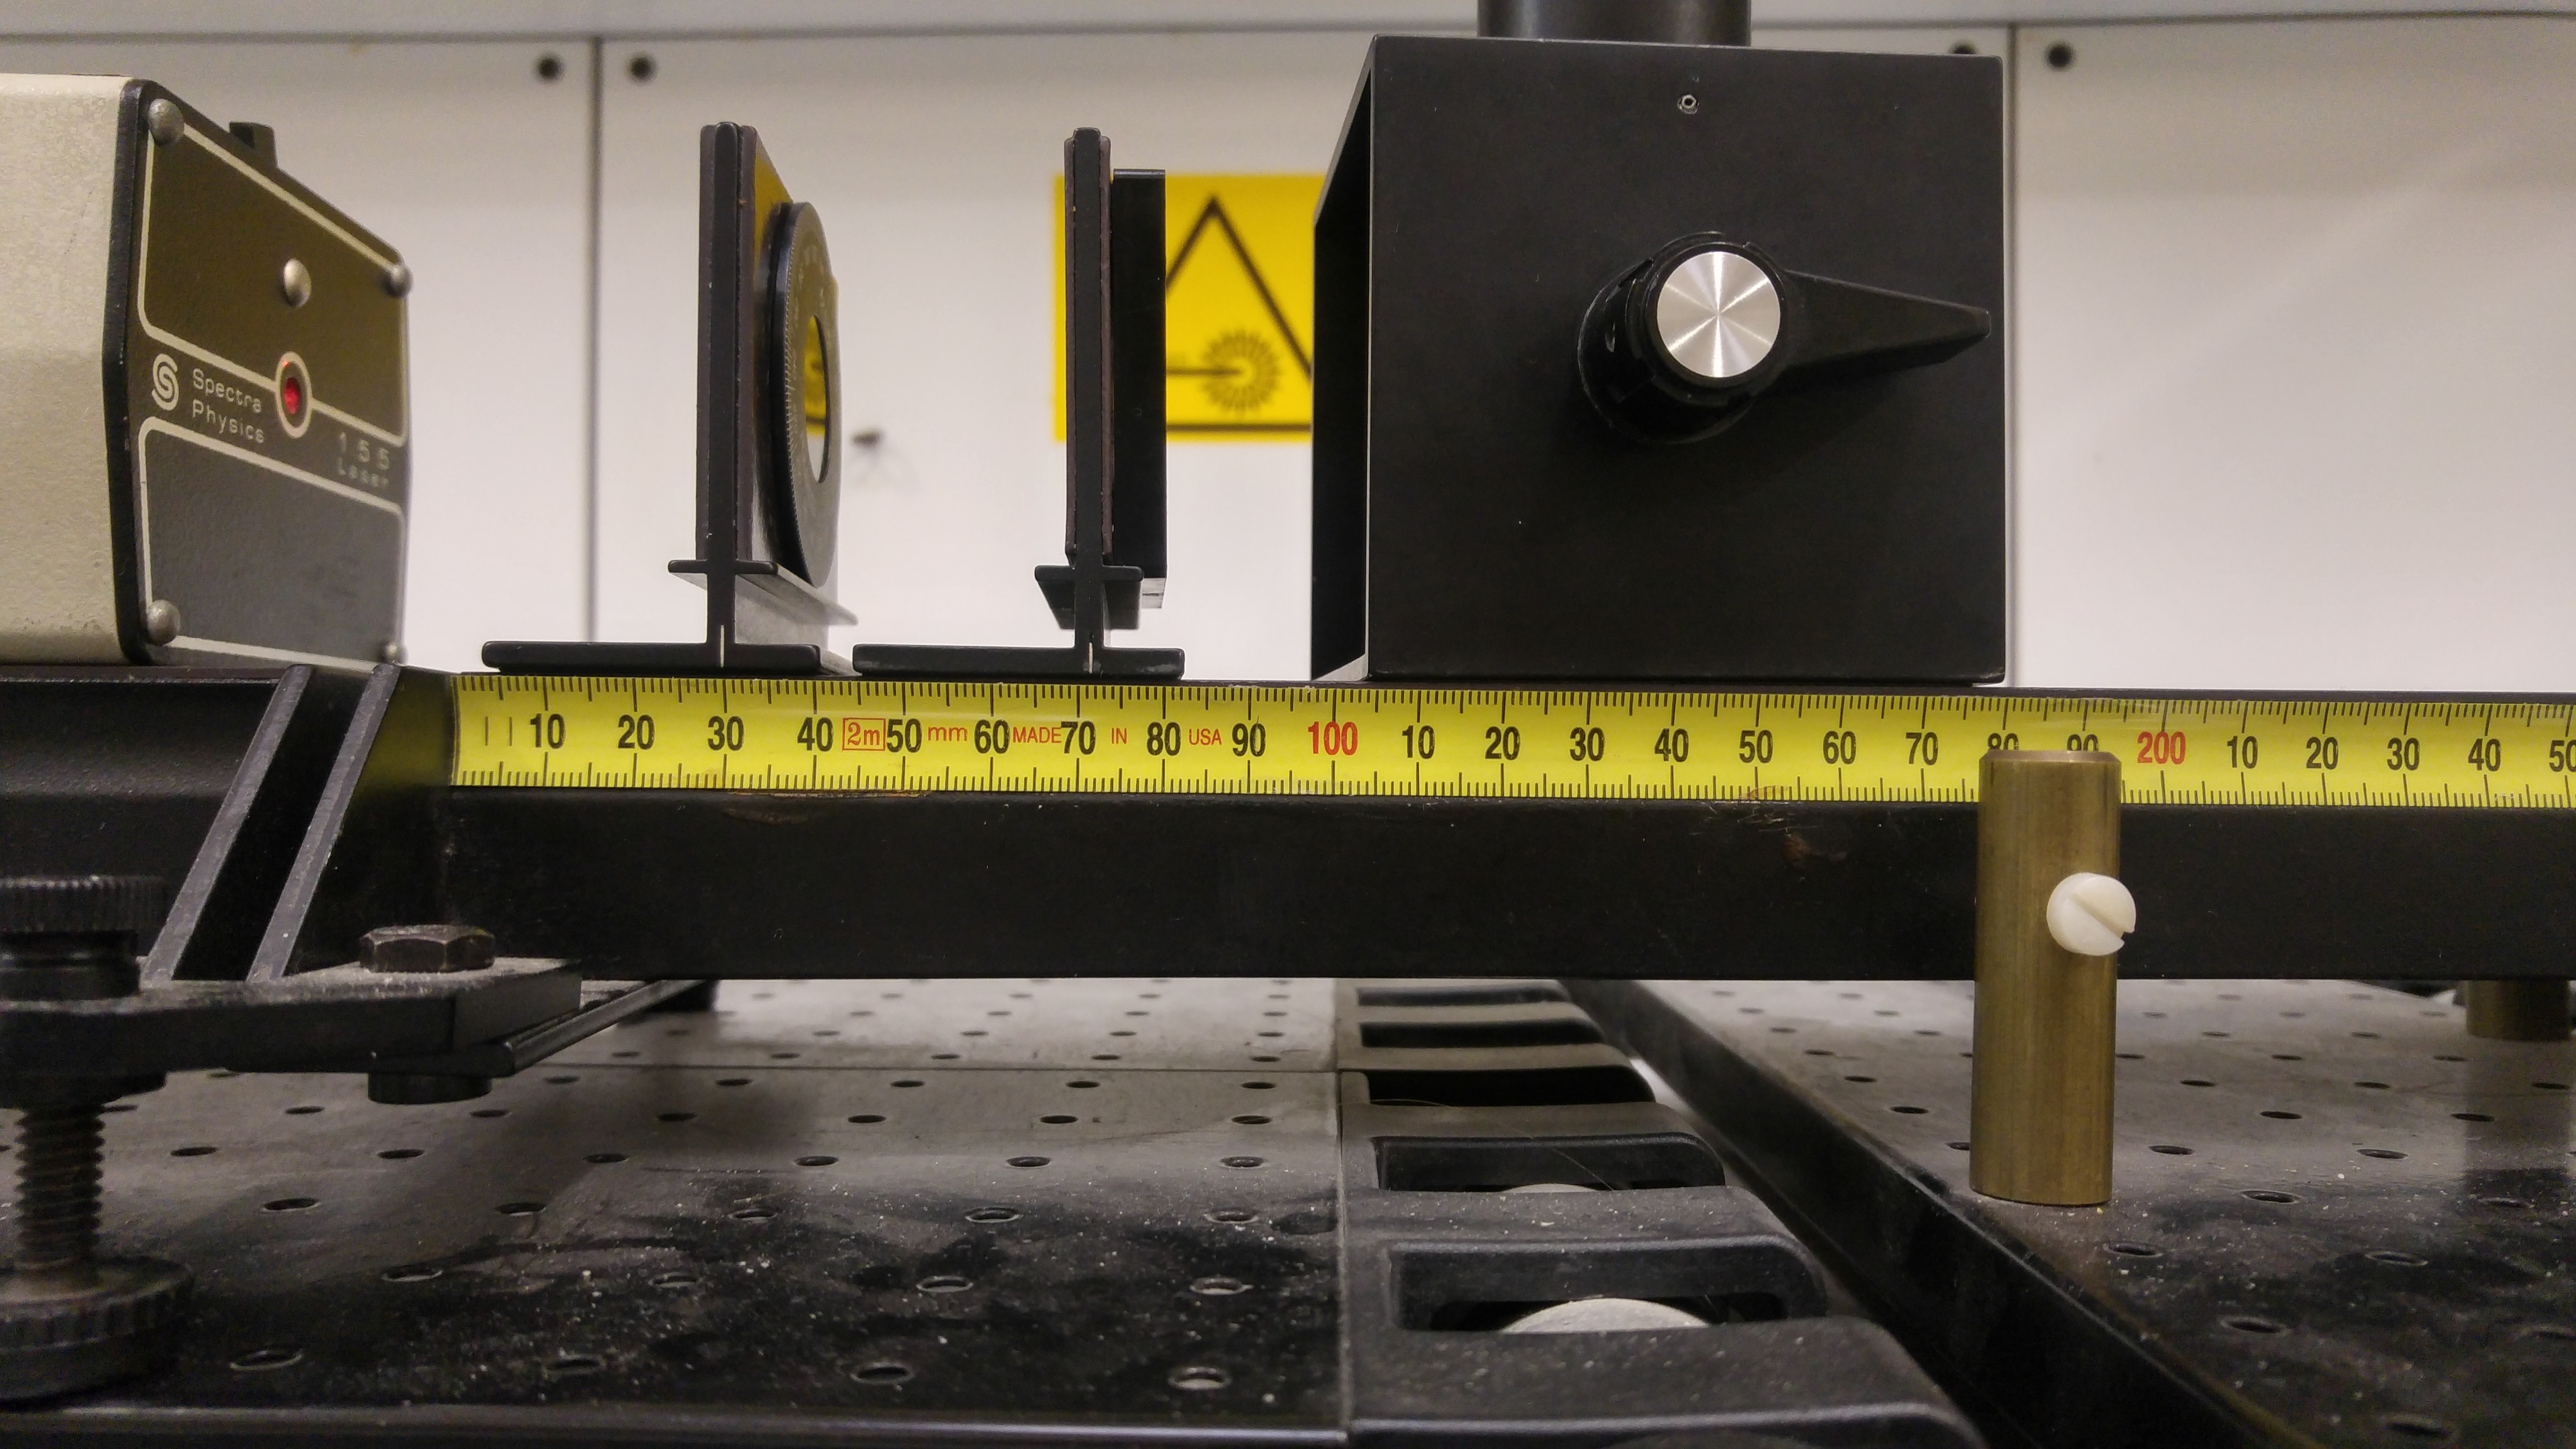
\includegraphics[]{/VelLuce/Relazione/Immagini/photo4.jpg}    
		\caption{Disposizione dello splitter e delle lenti sulla scala graduata.}\label{photo4}
	\end{figure}
\subsection{Procedure di Misura Sperimentale}



La presa dati è consistita nella raccolta di una serie di differenze di distanze relative alla posizione del \textit{waist} sull oculare  -- opportunamente dotato di un mirino a X per centrare il \textit{waist} stesso, in quanto la posizione del punto rosso è dipendente dalla frequenza con cui lo specchio rotante viene fatto oscillare, come mostra l'equazione \ref{eqn:c}. La procedura sperimentale di misura consiste in una ripetizione dei seguenti passi:

\begin{itemize}
	\item Il motore è stato azionato a una frequenza relativamente bassa ($50-100$ Hz) ed è stata centrata la posizione del \textit{waist} muovendo la vite micrometrica.
	\item \'E stato registrato il valore della posizione individuato dal nonio collegato alla vite micrometrica.
	\item La frequenza di rotazione del motore è stata aumentata da $900-1000$ Hz fino anche al massimo, ed stata centrata la posizione del \textit{waist} muovendo la vite micrometrica.
	\item Di nuovo è stato registrato il valore della posizione tramite il nonio.
\end{itemize}

Questa ripetizione viene eseguita per entrambi i sensi in cui il motore è in grado di imprimere rotazione alla cinghia (\textit{clockwise} e \textit{counterclockwise}). Inoltre è stato possibile eseguire delle misure anche tra massimo \textit{clockwise} e massimo \textit{counterclockwise} avendo cura di fermare il motore senza passare immediatamente da un senso di rotazione all'altro. La ripetizione di misure indipendenti tra loro consente poi di eseguire analisi statistica sui campioni di dati estratti.

In questa sede va fatto notare un problema riscontrato durante le operazioni di misura: Non è stato possibile individuare se il problema fosse relativo al motore, o al display che segnalava la frequenza di rotazione, ma quello che si osservava era la poca stabilità nel numero di Hz segnalati. Come conseguenza di questo fatto è risultato difficile eseguire 20-30 misure per ogni set di dati (specie considerando che la massima frequenza del motorino aveva un'autonomia di un minuto circa e spesso il display non si era ancora stabilizzato). Abbiamo fatto in modo di effetturare il maggior numero di misure possibili compatibilmente con i tempi richiesti per effettuare una misura (spesso oltre un minuto per attendere che il display fosse stabile).

\end{document}